% !TEX root = master.tex

% Questions and answers by Vivek Shah

\questionhead{Computer Networks}{80 minutes}
\subquestionhead{True/False Questions}{8 minutes}
\begin{tfquestion}
\tfitem[true]{Implementation of link layer protocols span both hardware (network controllers) and software (operating systems).}
\tfitem[true]{Peer-to-peer architectures exhibit better scalability because adding peers results in an increase in cumulative bandwidth available for all communicating parties.}
\tfitem[false]{For a TCP connection, the receive window can never become zero.}
\tfitem[true]{Convergence time of OSPF protocol is independent of the number of edges in a network.}
\end{tfquestion}

\subquestionhead{Multiple Choice Questions}{15 minutes}
\emph{In each of the following questions choose one answer.}

\begin{mcquestion}
Consider a two dimensional even parity scheme for error detection. Using this scheme compute the parity bits of the 8-bit ASCII\footnote{ASCII codes of A-Z lie contiguously between decimal numbers 65-90.} representation of "REEXAM" where each byte of the word forms a row for the two dimensional parity scheme. The resultant parity bits (row followed by column parity bits) are
\mcitem[check]{111100 00000110}
\mcitem{111101 00000010}
\mcitem{100101 00001110}
\mcitem{None of the above}
\end{mcquestion}

\begin{mcquestion}
The broadcast address of the network 117.18.31.54/18 is 
\mcitem{117.18.31.255}
\mcitem[check]{117.18.63.255}
\mcitem{117.18.127.255}
\mcitem{None of the above}
\end{mcquestion}

\clearpage 
\subquestionhead{Short Questions}{24 minutes}

\begin{question}
Why is an ARP query sent within a broadcast frame while the ARP response is sent within a frame having a specific destination address?
\vspace{-2ex}
\answerlines[An ARP query is sent to resolve an IP address to a
MAC address by the link layer. Since the destination MAC address
is unknown, a link layer frame consisting of the ARP query is
broadcast using the special MAC broadcast address. Since an ARP
response is sent on receipt of an ARP query which contains the MAC
address of the sender, the link layer frame containing the ARP
response can be sent to the specific MAC address of the ARP query sender.]{12}
\end{question}

\clearpage

\subquestionhead{Network Routing}{18 minutes}
Consider the network topology outlined in the graph below

\begin{center}
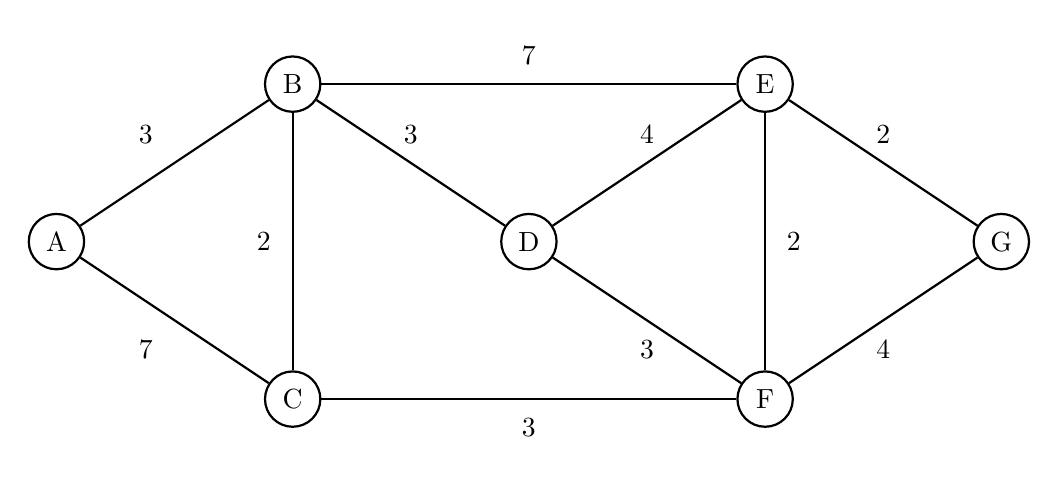
\begin{tikzpicture}[thick,minimum size=20pt,]
    \node[shape=circle,draw=black] (A) at (0,0) {A};
    \node[shape=circle,draw=black] (B) at (3,2) {B};
    \node[shape=circle,draw=black] (C) at (3,-2) {C};
    \node[shape=circle,draw=black] (D) at (6,0) {D};
    \node[shape=circle,draw=black] (E) at (9,2) {E};
    \node[shape=circle,draw=black] (F) at (9,-2) {F};
    \node[shape=circle,draw=black] (G) at (12,0) {G};
    \path [-](A) edge node[above left]{$3$} (B);
    \path [-](A) edge node[below left]{$7$} (C);
    \path [-](B) edge node[left]{$2$} (C);
    \path [-](B) edge node[above]{$3$} (D);
    %\path [-](C) edge node[below]{$4$} (D);
    \path [-](D) edge node[above]{$4$} (E);
    \path [-](D) edge node[below]{$3$} (F);
    \path [-](B) edge node[above]{$7$} (E);
    \path [-](C) edge node[below]{$3$} (F);
    \path [-](E) edge node[above]{$2$} (G);
    \path [-](E) edge node[right]{$2$} (F);
    \path [-](F) edge node[below]{$4$} (G);
\end{tikzpicture}
\end{center}

\begin{question}
Apply the link state routing algorithm and compute the forwarding tables on nodes A and D. (Note: Remember to show the steps of the algorithm.)\\
\answerfigure[The computation of link state routing algorithm
on node A:\\ \\
\begin{tabular}{|c|c|c|c|c|c|c|c|}
\hline
  Step & N' & D(B),p(B) & D(C),p(C) & D(D),p(D) & D(E),p(E) & D(F),p(F) & D(G),p(G) \\ \hline
  0 & A & 3,A & 7,A & $\infty$ & $\infty$ & $\infty$ & $\infty$ \\ \hline
  1 & AB &  & 5,B & 6,B & 10,B &  &  \\ \hline
  2 & ABC &  &  &  &  & 8,C &  \\ \hline
  3 & ABCD &  &  &  & 10,D/B & 8,C & \\ \hline
  4 & ABCDF &  &  &  & 10,D/B/F &  & 12,F \\ \hline
  5 & ABCDFE & & & & & & 12,F/E \\ \hline
  6 & ABCDFEG & & & & & & \\ \hline
\end{tabular}\\ \\
In the above computation, if there are multiple paths with same
cost they have been shown with / to demarcate them being
acceptable values. \\ \\
The computation of link state algorithm on node D:\\ \\
\begin{tabular}{|c|c|c|c|c|c|c|c|}
\hline
  Step & N' & D(A),p(A) & D(B),p(B) & D(C),p(C) & D(E),p(E) & D(F),p(F) & D(G),p(G) \\ \hline
  0 & D & $\infty$ & 3,D & $\infty$ & 4,D & 3,D & $\infty$ \\ \hline
  1 & DB & 6,B &  & 5,B & 4,D &  &  \\ \hline
  2 & DBF &  &  & 5,B & 4,D & & 7,F \\ \hline
  3 & DBFE &  &  &  &  & 3,D & 6,E \\ \hline
  4 & DBFEC & 6,B &  &  &  &  &  \\ \hline
  5 & DBFECA & & & & & & \\ \hline
  6 & DBFECAG & & & & & & \\ \hline
\end{tabular}\\ \\
In the above computation because of equal cost paths existing the
choice of nodes in N' can be inverted in step 1 and 2 and in steps
5 and 6.]{14cm}
\answerfigure[Forwarding table on node A follows:\\ \\
\begin{tabular}{|c|c|}
  \hline
  Destination node & Edge \\ \hline
  all nodes & (A,B) \\ \hline
\end{tabular} \\ \\ \\ \\
Forwarding table on node D follows:\\ \\
\begin{tabular}{|c|c|}
  \hline
  Destination node & Edge \\ \hline
  A & (D,B) \\ \hline
  B & (D,B) \\ \hline
  C & (D,B) \\ \hline
  E & (D,E) \\ \hline
  F & (D,F) \\ \hline
  G & (D,E) \\ \hline
\end{tabular}]{10cm}
\end{question}

\begin{question}
List the problems that are overcome using hierarchical routing.
\vspace{-3ex}
\answerlines[Some of the problems that are solved by hierarchical
routing are: \\
1. Scalability issues in message communication overheads with
growing network size.\\
2. Scalability issues in routing algorithm computing overheads
with growing network size.\\
3. Scalability issues in storage and retrieval overheads of
routing information with growing network size. \\
2. Administrative autonomy which allows each autonomous network to
operate and administer itself while still being able to
inter-operate with other networks.]{12}
\end{question}


